\documentclass{article} % For LaTeX2e
\usepackage{iclr2022_conference,times}
% Optional math commands from https://github.com/goodfeli/dlbook_notation.
%%%%% NEW MATH DEFINITIONS %%%%%

\usepackage{amsmath,amsfonts,bm}

% Mark sections of captions for referring to divisions of figures
\newcommand{\figleft}{{\em (Left)}}
\newcommand{\figcenter}{{\em (Center)}}
\newcommand{\figright}{{\em (Right)}}
\newcommand{\figtop}{{\em (Top)}}
\newcommand{\figbottom}{{\em (Bottom)}}
\newcommand{\captiona}{{\em (a)}}
\newcommand{\captionb}{{\em (b)}}
\newcommand{\captionc}{{\em (c)}}
\newcommand{\captiond}{{\em (d)}}

% Highlight a newly defined term
\newcommand{\newterm}[1]{{\bf #1}}


% Figure reference, lower-case.
\def\figref#1{figure~\ref{#1}}
% Figure reference, capital. For start of sentence
\def\Figref#1{Figure~\ref{#1}}
\def\twofigref#1#2{figures \ref{#1} and \ref{#2}}
\def\quadfigref#1#2#3#4{figures \ref{#1}, \ref{#2}, \ref{#3} and \ref{#4}}
% Section reference, lower-case.
\def\secref#1{section~\ref{#1}}
% Section reference, capital.
\def\Secref#1{Section~\ref{#1}}
% Reference to two sections.
\def\twosecrefs#1#2{sections \ref{#1} and \ref{#2}}
% Reference to three sections.
\def\secrefs#1#2#3{sections \ref{#1}, \ref{#2} and \ref{#3}}
% Reference to an equation, lower-case.
\def\eqref#1{equation~\ref{#1}}
% Reference to an equation, upper case
\def\Eqref#1{Equation~\ref{#1}}
% A raw reference to an equation---avoid using if possible
\def\plaineqref#1{\ref{#1}}
% Reference to a chapter, lower-case.
\def\chapref#1{chapter~\ref{#1}}
% Reference to an equation, upper case.
\def\Chapref#1{Chapter~\ref{#1}}
% Reference to a range of chapters
\def\rangechapref#1#2{chapters\ref{#1}--\ref{#2}}
% Reference to an algorithm, lower-case.
\def\algref#1{algorithm~\ref{#1}}
% Reference to an algorithm, upper case.
\def\Algref#1{Algorithm~\ref{#1}}
\def\twoalgref#1#2{algorithms \ref{#1} and \ref{#2}}
\def\Twoalgref#1#2{Algorithms \ref{#1} and \ref{#2}}
% Reference to a part, lower case
\def\partref#1{part~\ref{#1}}
% Reference to a part, upper case
\def\Partref#1{Part~\ref{#1}}
\def\twopartref#1#2{parts \ref{#1} and \ref{#2}}

\def\ceil#1{\lceil #1 \rceil}
\def\floor#1{\lfloor #1 \rfloor}
\def\1{\bm{1}}
\newcommand{\train}{\mathcal{D}}
\newcommand{\valid}{\mathcal{D_{\mathrm{valid}}}}
\newcommand{\test}{\mathcal{D_{\mathrm{test}}}}

\def\eps{{\epsilon}}


% Random variables
\def\reta{{\textnormal{$\eta$}}}
\def\ra{{\textnormal{a}}}
\def\rb{{\textnormal{b}}}
\def\rc{{\textnormal{c}}}
\def\rd{{\textnormal{d}}}
\def\re{{\textnormal{e}}}
\def\rf{{\textnormal{f}}}
\def\rg{{\textnormal{g}}}
\def\rh{{\textnormal{h}}}
\def\ri{{\textnormal{i}}}
\def\rj{{\textnormal{j}}}
\def\rk{{\textnormal{k}}}
\def\rl{{\textnormal{l}}}
% rm is already a command, just don't name any random variables m
\def\rn{{\textnormal{n}}}
\def\ro{{\textnormal{o}}}
\def\rp{{\textnormal{p}}}
\def\rq{{\textnormal{q}}}
\def\rr{{\textnormal{r}}}
\def\rs{{\textnormal{s}}}
\def\rt{{\textnormal{t}}}
\def\ru{{\textnormal{u}}}
\def\rv{{\textnormal{v}}}
\def\rw{{\textnormal{w}}}
\def\rx{{\textnormal{x}}}
\def\ry{{\textnormal{y}}}
\def\rz{{\textnormal{z}}}

% Random vectors
\def\rvepsilon{{\mathbf{\epsilon}}}
\def\rvtheta{{\mathbf{\theta}}}
\def\rva{{\mathbf{a}}}
\def\rvb{{\mathbf{b}}}
\def\rvc{{\mathbf{c}}}
\def\rvd{{\mathbf{d}}}
\def\rve{{\mathbf{e}}}
\def\rvf{{\mathbf{f}}}
\def\rvg{{\mathbf{g}}}
\def\rvh{{\mathbf{h}}}
\def\rvu{{\mathbf{i}}}
\def\rvj{{\mathbf{j}}}
\def\rvk{{\mathbf{k}}}
\def\rvl{{\mathbf{l}}}
\def\rvm{{\mathbf{m}}}
\def\rvn{{\mathbf{n}}}
\def\rvo{{\mathbf{o}}}
\def\rvp{{\mathbf{p}}}
\def\rvq{{\mathbf{q}}}
\def\rvr{{\mathbf{r}}}
\def\rvs{{\mathbf{s}}}
\def\rvt{{\mathbf{t}}}
\def\rvu{{\mathbf{u}}}
\def\rvv{{\mathbf{v}}}
\def\rvw{{\mathbf{w}}}
\def\rvx{{\mathbf{x}}}
\def\rvy{{\mathbf{y}}}
\def\rvz{{\mathbf{z}}}

% Elements of random vectors
\def\erva{{\textnormal{a}}}
\def\ervb{{\textnormal{b}}}
\def\ervc{{\textnormal{c}}}
\def\ervd{{\textnormal{d}}}
\def\erve{{\textnormal{e}}}
\def\ervf{{\textnormal{f}}}
\def\ervg{{\textnormal{g}}}
\def\ervh{{\textnormal{h}}}
\def\ervi{{\textnormal{i}}}
\def\ervj{{\textnormal{j}}}
\def\ervk{{\textnormal{k}}}
\def\ervl{{\textnormal{l}}}
\def\ervm{{\textnormal{m}}}
\def\ervn{{\textnormal{n}}}
\def\ervo{{\textnormal{o}}}
\def\ervp{{\textnormal{p}}}
\def\ervq{{\textnormal{q}}}
\def\ervr{{\textnormal{r}}}
\def\ervs{{\textnormal{s}}}
\def\ervt{{\textnormal{t}}}
\def\ervu{{\textnormal{u}}}
\def\ervv{{\textnormal{v}}}
\def\ervw{{\textnormal{w}}}
\def\ervx{{\textnormal{x}}}
\def\ervy{{\textnormal{y}}}
\def\ervz{{\textnormal{z}}}

% Random matrices
\def\rmA{{\mathbf{A}}}
\def\rmB{{\mathbf{B}}}
\def\rmC{{\mathbf{C}}}
\def\rmD{{\mathbf{D}}}
\def\rmE{{\mathbf{E}}}
\def\rmF{{\mathbf{F}}}
\def\rmG{{\mathbf{G}}}
\def\rmH{{\mathbf{H}}}
\def\rmI{{\mathbf{I}}}
\def\rmJ{{\mathbf{J}}}
\def\rmK{{\mathbf{K}}}
\def\rmL{{\mathbf{L}}}
\def\rmM{{\mathbf{M}}}
\def\rmN{{\mathbf{N}}}
\def\rmO{{\mathbf{O}}}
\def\rmP{{\mathbf{P}}}
\def\rmQ{{\mathbf{Q}}}
\def\rmR{{\mathbf{R}}}
\def\rmS{{\mathbf{S}}}
\def\rmT{{\mathbf{T}}}
\def\rmU{{\mathbf{U}}}
\def\rmV{{\mathbf{V}}}
\def\rmW{{\mathbf{W}}}
\def\rmX{{\mathbf{X}}}
\def\rmY{{\mathbf{Y}}}
\def\rmZ{{\mathbf{Z}}}

% Elements of random matrices
\def\ermA{{\textnormal{A}}}
\def\ermB{{\textnormal{B}}}
\def\ermC{{\textnormal{C}}}
\def\ermD{{\textnormal{D}}}
\def\ermE{{\textnormal{E}}}
\def\ermF{{\textnormal{F}}}
\def\ermG{{\textnormal{G}}}
\def\ermH{{\textnormal{H}}}
\def\ermI{{\textnormal{I}}}
\def\ermJ{{\textnormal{J}}}
\def\ermK{{\textnormal{K}}}
\def\ermL{{\textnormal{L}}}
\def\ermM{{\textnormal{M}}}
\def\ermN{{\textnormal{N}}}
\def\ermO{{\textnormal{O}}}
\def\ermP{{\textnormal{P}}}
\def\ermQ{{\textnormal{Q}}}
\def\ermR{{\textnormal{R}}}
\def\ermS{{\textnormal{S}}}
\def\ermT{{\textnormal{T}}}
\def\ermU{{\textnormal{U}}}
\def\ermV{{\textnormal{V}}}
\def\ermW{{\textnormal{W}}}
\def\ermX{{\textnormal{X}}}
\def\ermY{{\textnormal{Y}}}
\def\ermZ{{\textnormal{Z}}}

% Vectors
\def\vzero{{\bm{0}}}
\def\vone{{\bm{1}}}
\def\vmu{{\bm{\mu}}}
\def\vtheta{{\bm{\theta}}}
\def\va{{\bm{a}}}
\def\vb{{\bm{b}}}
\def\vc{{\bm{c}}}
\def\vd{{\bm{d}}}
\def\ve{{\bm{e}}}
\def\vf{{\bm{f}}}
\def\vg{{\bm{g}}}
\def\vh{{\bm{h}}}
\def\vi{{\bm{i}}}
\def\vj{{\bm{j}}}
\def\vk{{\bm{k}}}
\def\vl{{\bm{l}}}
\def\vm{{\bm{m}}}
\def\vn{{\bm{n}}}
\def\vo{{\bm{o}}}
\def\vp{{\bm{p}}}
\def\vq{{\bm{q}}}
\def\vr{{\bm{r}}}
\def\vs{{\bm{s}}}
\def\vt{{\bm{t}}}
\def\vu{{\bm{u}}}
\def\vv{{\bm{v}}}
\def\vw{{\bm{w}}}
\def\vx{{\bm{x}}}
\def\vy{{\bm{y}}}
\def\vz{{\bm{z}}}

% Elements of vectors
\def\evalpha{{\alpha}}
\def\evbeta{{\beta}}
\def\evepsilon{{\epsilon}}
\def\evlambda{{\lambda}}
\def\evomega{{\omega}}
\def\evmu{{\mu}}
\def\evpsi{{\psi}}
\def\evsigma{{\sigma}}
\def\evtheta{{\theta}}
\def\eva{{a}}
\def\evb{{b}}
\def\evc{{c}}
\def\evd{{d}}
\def\eve{{e}}
\def\evf{{f}}
\def\evg{{g}}
\def\evh{{h}}
\def\evi{{i}}
\def\evj{{j}}
\def\evk{{k}}
\def\evl{{l}}
\def\evm{{m}}
\def\evn{{n}}
\def\evo{{o}}
\def\evp{{p}}
\def\evq{{q}}
\def\evr{{r}}
\def\evs{{s}}
\def\evt{{t}}
\def\evu{{u}}
\def\evv{{v}}
\def\evw{{w}}
\def\evx{{x}}
\def\evy{{y}}
\def\evz{{z}}

% Matrix
\def\mA{{\bm{A}}}
\def\mB{{\bm{B}}}
\def\mC{{\bm{C}}}
\def\mD{{\bm{D}}}
\def\mE{{\bm{E}}}
\def\mF{{\bm{F}}}
\def\mG{{\bm{G}}}
\def\mH{{\bm{H}}}
\def\mI{{\bm{I}}}
\def\mJ{{\bm{J}}}
\def\mK{{\bm{K}}}
\def\mL{{\bm{L}}}
\def\mM{{\bm{M}}}
\def\mN{{\bm{N}}}
\def\mO{{\bm{O}}}
\def\mP{{\bm{P}}}
\def\mQ{{\bm{Q}}}
\def\mR{{\bm{R}}}
\def\mS{{\bm{S}}}
\def\mT{{\bm{T}}}
\def\mU{{\bm{U}}}
\def\mV{{\bm{V}}}
\def\mW{{\bm{W}}}
\def\mX{{\bm{X}}}
\def\mY{{\bm{Y}}}
\def\mZ{{\bm{Z}}}
\def\mBeta{{\bm{\beta}}}
\def\mPhi{{\bm{\Phi}}}
\def\mLambda{{\bm{\Lambda}}}
\def\mSigma{{\bm{\Sigma}}}

% Tensor
\DeclareMathAlphabet{\mathsfit}{\encodingdefault}{\sfdefault}{m}{sl}
\SetMathAlphabet{\mathsfit}{bold}{\encodingdefault}{\sfdefault}{bx}{n}
\newcommand{\tens}[1]{\bm{\mathsfit{#1}}}
\def\tA{{\tens{A}}}
\def\tB{{\tens{B}}}
\def\tC{{\tens{C}}}
\def\tD{{\tens{D}}}
\def\tE{{\tens{E}}}
\def\tF{{\tens{F}}}
\def\tG{{\tens{G}}}
\def\tH{{\tens{H}}}
\def\tI{{\tens{I}}}
\def\tJ{{\tens{J}}}
\def\tK{{\tens{K}}}
\def\tL{{\tens{L}}}
\def\tM{{\tens{M}}}
\def\tN{{\tens{N}}}
\def\tO{{\tens{O}}}
\def\tP{{\tens{P}}}
\def\tQ{{\tens{Q}}}
\def\tR{{\tens{R}}}
\def\tS{{\tens{S}}}
\def\tT{{\tens{T}}}
\def\tU{{\tens{U}}}
\def\tV{{\tens{V}}}
\def\tW{{\tens{W}}}
\def\tX{{\tens{X}}}
\def\tY{{\tens{Y}}}
\def\tZ{{\tens{Z}}}


% Graph
\def\gA{{\mathcal{A}}}
\def\gB{{\mathcal{B}}}
\def\gC{{\mathcal{C}}}
\def\gD{{\mathcal{D}}}
\def\gE{{\mathcal{E}}}
\def\gF{{\mathcal{F}}}
\def\gG{{\mathcal{G}}}
\def\gH{{\mathcal{H}}}
\def\gI{{\mathcal{I}}}
\def\gJ{{\mathcal{J}}}
\def\gK{{\mathcal{K}}}
\def\gL{{\mathcal{L}}}
\def\gM{{\mathcal{M}}}
\def\gN{{\mathcal{N}}}
\def\gO{{\mathcal{O}}}
\def\gP{{\mathcal{P}}}
\def\gQ{{\mathcal{Q}}}
\def\gR{{\mathcal{R}}}
\def\gS{{\mathcal{S}}}
\def\gT{{\mathcal{T}}}
\def\gU{{\mathcal{U}}}
\def\gV{{\mathcal{V}}}
\def\gW{{\mathcal{W}}}
\def\gX{{\mathcal{X}}}
\def\gY{{\mathcal{Y}}}
\def\gZ{{\mathcal{Z}}}

% Sets
\def\sA{{\mathbb{A}}}
\def\sB{{\mathbb{B}}}
\def\sC{{\mathbb{C}}}
\def\sD{{\mathbb{D}}}
% Don't use a set called E, because this would be the same as our symbol
% for expectation.
\def\sF{{\mathbb{F}}}
\def\sG{{\mathbb{G}}}
\def\sH{{\mathbb{H}}}
\def\sI{{\mathbb{I}}}
\def\sJ{{\mathbb{J}}}
\def\sK{{\mathbb{K}}}
\def\sL{{\mathbb{L}}}
\def\sM{{\mathbb{M}}}
\def\sN{{\mathbb{N}}}
\def\sO{{\mathbb{O}}}
\def\sP{{\mathbb{P}}}
\def\sQ{{\mathbb{Q}}}
\def\sR{{\mathbb{R}}}
\def\sS{{\mathbb{S}}}
\def\sT{{\mathbb{T}}}
\def\sU{{\mathbb{U}}}
\def\sV{{\mathbb{V}}}
\def\sW{{\mathbb{W}}}
\def\sX{{\mathbb{X}}}
\def\sY{{\mathbb{Y}}}
\def\sZ{{\mathbb{Z}}}

% Entries of a matrix
\def\emLambda{{\Lambda}}
\def\emA{{A}}
\def\emB{{B}}
\def\emC{{C}}
\def\emD{{D}}
\def\emE{{E}}
\def\emF{{F}}
\def\emG{{G}}
\def\emH{{H}}
\def\emI{{I}}
\def\emJ{{J}}
\def\emK{{K}}
\def\emL{{L}}
\def\emM{{M}}
\def\emN{{N}}
\def\emO{{O}}
\def\emP{{P}}
\def\emQ{{Q}}
\def\emR{{R}}
\def\emS{{S}}
\def\emT{{T}}
\def\emU{{U}}
\def\emV{{V}}
\def\emW{{W}}
\def\emX{{X}}
\def\emY{{Y}}
\def\emZ{{Z}}
\def\emSigma{{\Sigma}}

% entries of a tensor
% Same font as tensor, without \bm wrapper
\newcommand{\etens}[1]{\mathsfit{#1}}
\def\etLambda{{\etens{\Lambda}}}
\def\etA{{\etens{A}}}
\def\etB{{\etens{B}}}
\def\etC{{\etens{C}}}
\def\etD{{\etens{D}}}
\def\etE{{\etens{E}}}
\def\etF{{\etens{F}}}
\def\etG{{\etens{G}}}
\def\etH{{\etens{H}}}
\def\etI{{\etens{I}}}
\def\etJ{{\etens{J}}}
\def\etK{{\etens{K}}}
\def\etL{{\etens{L}}}
\def\etM{{\etens{M}}}
\def\etN{{\etens{N}}}
\def\etO{{\etens{O}}}
\def\etP{{\etens{P}}}
\def\etQ{{\etens{Q}}}
\def\etR{{\etens{R}}}
\def\etS{{\etens{S}}}
\def\etT{{\etens{T}}}
\def\etU{{\etens{U}}}
\def\etV{{\etens{V}}}
\def\etW{{\etens{W}}}
\def\etX{{\etens{X}}}
\def\etY{{\etens{Y}}}
\def\etZ{{\etens{Z}}}

% The true underlying data generating distribution
\newcommand{\pdata}{p_{\rm{data}}}
% The empirical distribution defined by the training set
\newcommand{\ptrain}{\hat{p}_{\rm{data}}}
\newcommand{\Ptrain}{\hat{P}_{\rm{data}}}
% The model distribution
\newcommand{\pmodel}{p_{\rm{model}}}
\newcommand{\Pmodel}{P_{\rm{model}}}
\newcommand{\ptildemodel}{\tilde{p}_{\rm{model}}}
% Stochastic autoencoder distributions
\newcommand{\pencode}{p_{\rm{encoder}}}
\newcommand{\pdecode}{p_{\rm{decoder}}}
\newcommand{\precons}{p_{\rm{reconstruct}}}

\newcommand{\laplace}{\mathrm{Laplace}} % Laplace distribution

\newcommand{\E}{\mathbb{E}}
\newcommand{\Ls}{\mathcal{L}}
\newcommand{\R}{\mathbb{R}}
\newcommand{\emp}{\tilde{p}}
\newcommand{\lr}{\alpha}
\newcommand{\reg}{\lambda}
\newcommand{\rect}{\mathrm{rectifier}}
\newcommand{\softmax}{\mathrm{softmax}}
\newcommand{\sigmoid}{\sigma}
\newcommand{\softplus}{\zeta}
\newcommand{\KL}{D_{\mathrm{KL}}}
\newcommand{\Var}{\mathrm{Var}}
\newcommand{\standarderror}{\mathrm{SE}}
\newcommand{\Cov}{\mathrm{Cov}}
% Wolfram Mathworld says $L^2$ is for function spaces and $\ell^2$ is for vectors
% But then they seem to use $L^2$ for vectors throughout the site, and so does
% wikipedia.
\newcommand{\normlzero}{L^0}
\newcommand{\normlone}{L^1}
\newcommand{\normltwo}{L^2}
\newcommand{\normlp}{L^p}
\newcommand{\normmax}{L^\infty}

\newcommand{\parents}{Pa} % See usage in notation.tex. Chosen to match Daphne's book.

\DeclareMathOperator*{\argmax}{arg\,max}
\DeclareMathOperator*{\argmin}{arg\,min}

\DeclareMathOperator{\sign}{sign}
\DeclareMathOperator{\Tr}{Tr}
\let\ab\allowbreak


%######## APS360: Uncomment your submission name
%\newcommand{\apsname}{Project Proposal}
%\newcommand{\apsname}{Progress Report}
\newcommand{\apsname}{Final Report}

%######## APS360: Put your Group Number here
\newcommand{\gpnumber}{28}

\usepackage{hyperref}
\usepackage{url}
\usepackage{graphicx}

%######## APS360: Put your project Title here
\title{Project Final Report: Traffic Sign Recognition Through Deep Learning}


%######## APS360: Put your names, student IDs and Emails here
\author{Salwa Waseem  \\
Student\# 1009021416\\
\texttt{salwa.waseem@mail.utoronto.ca} \\
\And
Maya Ramaneetharan Ramanathan  \\
Student\# 1008717596 \\
\texttt{maya.ramanathan@mail.utoronto.ca} \\
\AND
Maryah Noorani  \\
Student\# 1008343188 \\
\texttt{maryah.noorani@mail.utoronto.ca} \\
\And
Seoyeon (Sally) Kim \\
Student\# 1007713949 \\
\texttt{sysally.kim@mail.utoronto.ca} \\
\AND
}

% The \author macro works with any number of authors. There are two commands
% used to separate the names and addresses of multiple authors: \And and \AND.
%
% Using \And between authors leaves it to \LaTeX{} to determine where to break
% the lines. Using \AND forces a linebreak at that point. So, if \LaTeX{}
% puts 3 of 4 authors names on the first line, and the last on the second
% line, try using \AND instead of \And before the third author name.

\newcommand{\fix}{\marginpar{FIX}}
\newcommand{\new}{\marginpar{NEW}}

\iclrfinalcopy 
%######## APS360: Document starts here
\begin{document}


\maketitle

\begin{abstract}
The following document is the final report outlining the efforts of the Traffic Sign Recognition (TSR) project. To develop this model, a Convolutional Neural Network (CNN) has been developed to be able to classify various traffic signs from the German Traffic Sign Recognition Benchmark (GTSRB) dataset. This dataset is representative of universally used traffic signs, thus making it an optimal benchmark to test the model against. The final model has achieved high validation, test and training accuracy scores with the dataset used. This report presents and discusses the functionality and relevance of the TSR model created. 
%######## APS360: Do not change the next line. This shows your Main body page count.
----Total Pages: \pageref{last_page}
\end{abstract}



\section{Brief Project Description}
Rapid advancements in technology have generated cars which incorporate features designed to enhance driving safety. Traffic Sign Recognition (TSR) is a technology developed to improve road safety. TSR is employed in driver-assistance systems by automating detection of traffic signs; allowing cars to be adaptable to complex driving conditions. The responsiveness of vehicles to driving conditions will minimize human error, reducing road accidents and improving vehicle safety. 

Nevertheless, there is much to be desired in TSR as it faces challenges in diverse lighting conditions and unpleasant weather when it comes to maintaining high interpretation accuracy. Consequently, this project seeks to adapt TSR systems to handle complex driving scenarios while simultaneously conserving the recognition accuracy and computational efficiency. Deep learning models will be employed to amplify classification performance. These models will be trained to reliably identify traffic signs and will ultimately contribute to safer roads and smarter driving systems. 

\begin{figure}[h]
    \centering
    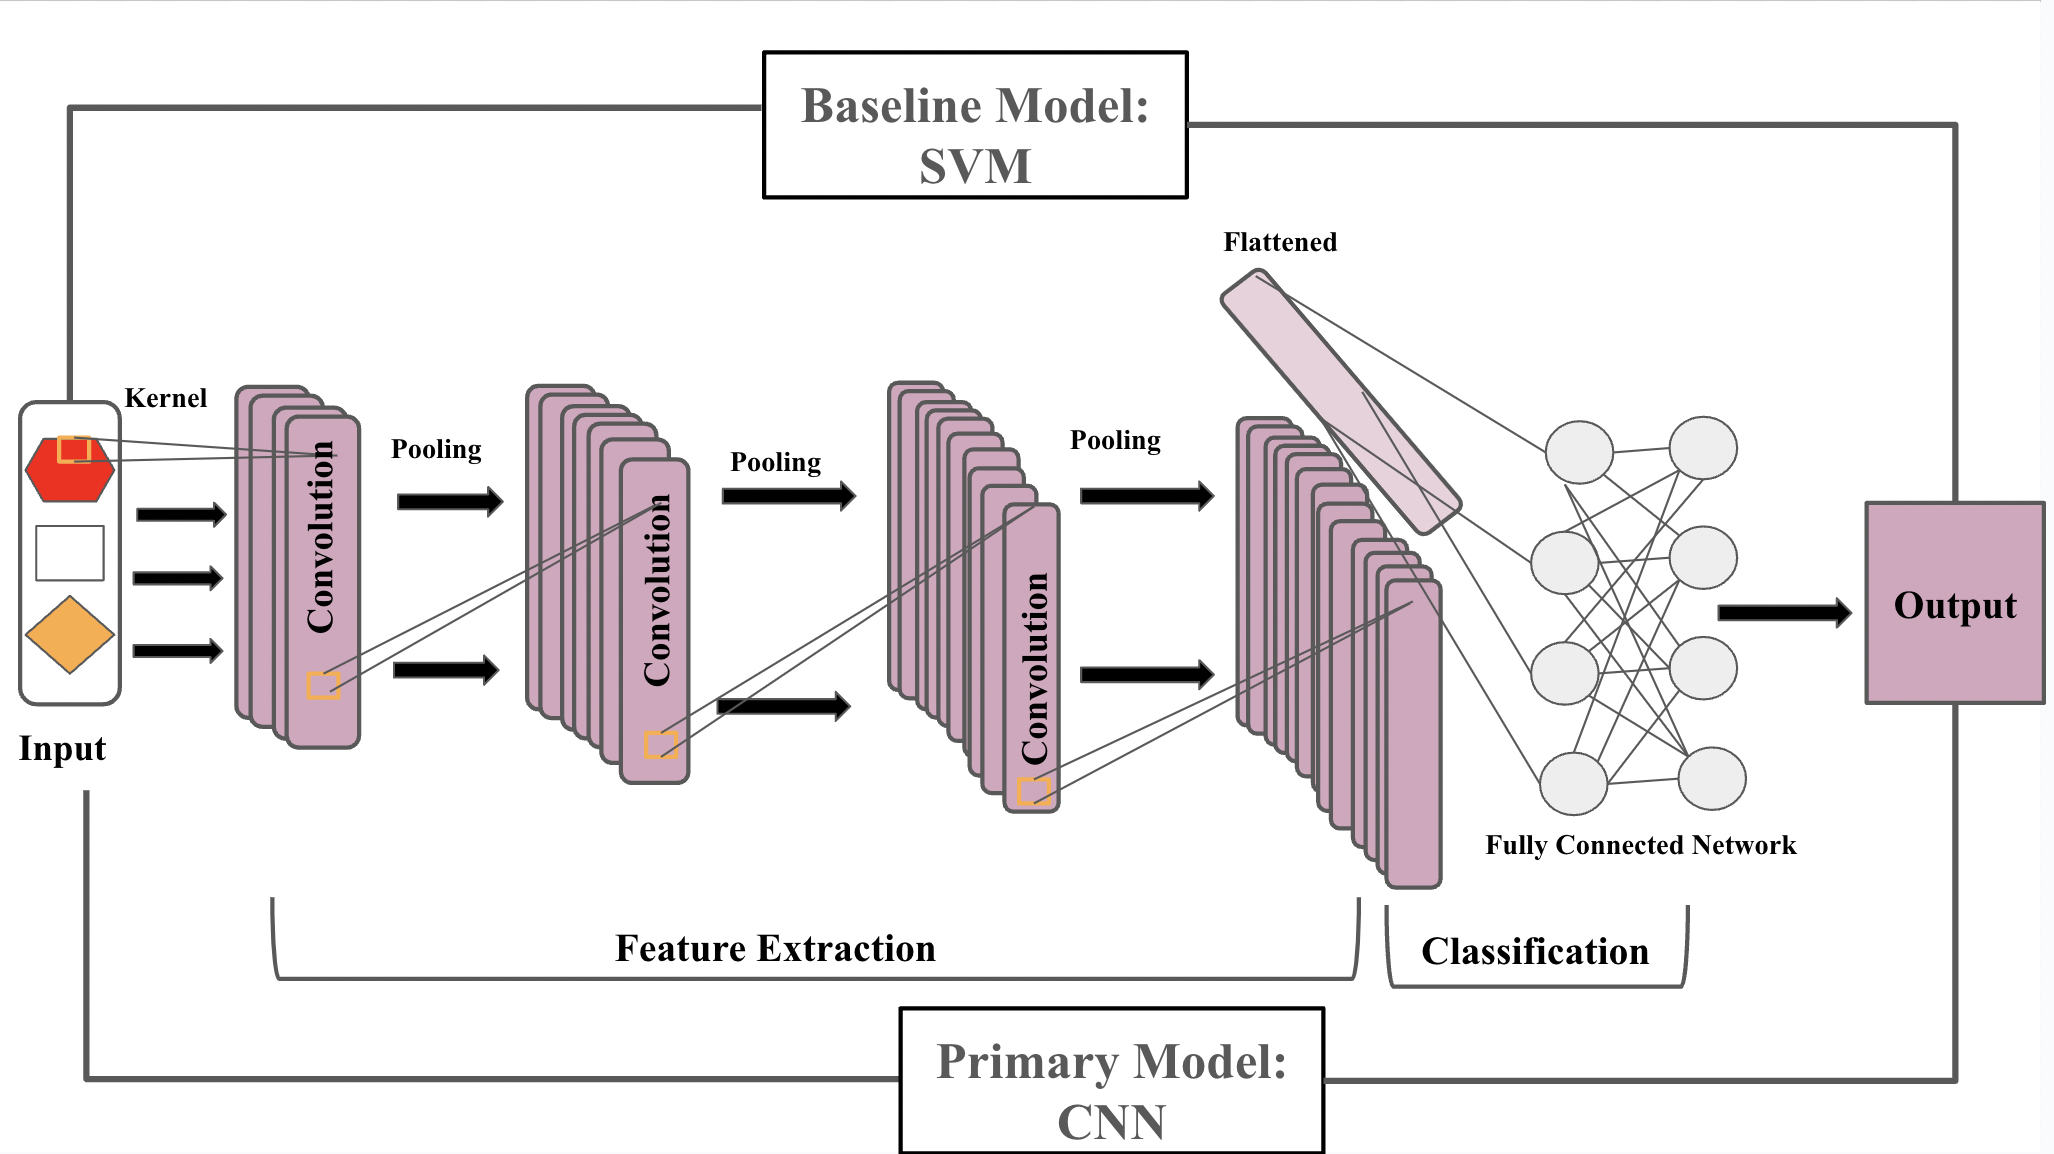
\includegraphics[width=0.5\linewidth]{project_desc1.png}
    \caption{Schematic of Deep Learning Model}
    \label{fig:enter-label}
\end{figure}

\section{Background and Related Work}
Several preceding studies have investigated methods for Traffic Sign Recognition (TSR), exhibiting the progression of techniques over the span of time. 

\citeauthor{Madani}(\citeyear{Madani}) developed a TSR model using Support Vector Machines (SVM), emphasizing pictogram features of traffic signs, yielding a recognition rate of 98.23\%. Similarly, \citeauthor{soni2019improving} (\citeyear{soni2019improving}) combined Histograms of Oriented Gradients (HOG), Local Binary Patterns (LBP), Principal Component Analysis (PCA), and SVM for traffic sign classification. PCA was employed to reduce the data dimensionality thus improving computational efficiency, yielding an accuracy of 84.45\%. \citeauthor{Namyang} (\citeyear{Namyang}) incorporated HOG, SVM, and Colour Layout Descriptors (CLD) in their model. Resizing traffic sign images to 120x80 pixels and employing an SVM and a Radial Basis Function (RBF) kernel achieved an accuracy of 93.98\%. On the other hand, \citeauthor{kerim} (\citeauthor{kerim}) examined the use of nine Artificial Neural Networks (ANNs) for TSR, with the combination of HOG and LBP for feature extraction. This method achieved an accuracy of 95\%, therefore outperforming models dependent solely on HOG. \citeauthor{li} (\citeyear{li}) utilized the German Traffic Sign Recognition Benchmark (GTSRB) to illustrate the advantages of incorporating colour histrograms, HOG, and PCA for dimensionality reduction. Their model has achieved a near-perfect accuracy of 99.99\%, highlighting the benefits of colour information and dimensionality reduction in the model.

Conventional methods exhibit high accuracy in very specific contexts and are dependent on feature engineering, hence struggling with generalization. Convolutional Neural Networks (CNN) tackle these limitations by automatically learning features from raw image data, therefore eliminating the need for manual extraction. CNNs also are adept at handling large and complex datasets and excel at capturing intricate patterns, hence being apt for TSR tasks. Leveraging the ability of deep learning to adapt to complex conditions, CNN-based models provide development over standard methods, particularly in scalability and classification accuracy. 

\section{Data Processing}

\subsection{Data Collection}
The data used in this model was obtained from the German Traffic Sign Recognition Benchmark (GTSRB) which contains pictures of traffic signs taken from the real world. This dataset includes images that vary in size, lighting and background conditions, simulating real-world scenarios.The images in this dataset come labeled, with each image associated with a specific traffic sign class.
\subsection{Data Preprocessing}
All the images going into the model are first preprocessed and standardized using the following steps:
\begin{figure}[h]
    \centering
    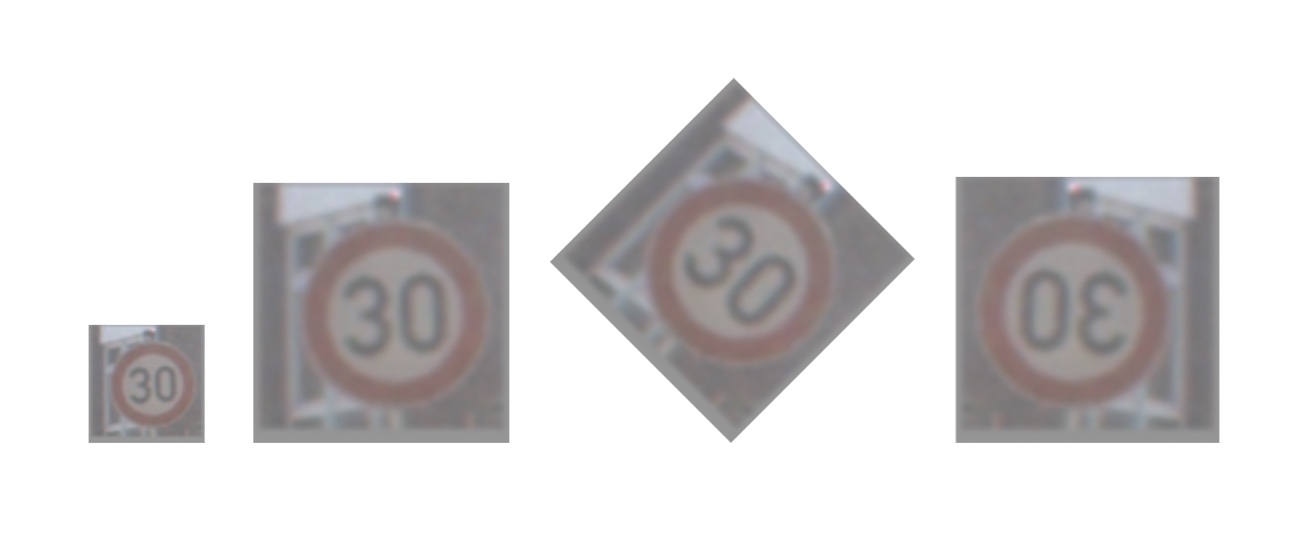
\includegraphics[width=0.5\linewidth]{Data Augmentation Images.jpg}
    \caption{
From left to right: Original image (59x59 pixels), Resized image (30x30 pixels), Data augmented image (Rotated by 45°), Flipped image
}
    \label{fig:enter-label}
\end{figure}

\begin{itemize}
    \item Resizing: All images are resized to a fixed dimension of 30x30 pixels to ensure uniformity in the input images going into the CNN.
    \item Normalization: The pixel values of each image are normalized to fall within the range [0,1] to ensure that the model focuses on all parts of the image equally and avoids bias.
    \item Augmentation: Augmentations such as brightness adjustments, zooms, rotations and flips are used to increase diversity while still preventing overfitting.
\end{itemize}

\subsection{Example Data}
This example image contains a speed limit sign at the center of the picture. According to the preprocessing procedures outlined above, this image is resized, normalized and augmented before being used as input for the model.

\label{headings}

\section{Architecture}
Our final neural network model for Traffic Sign Recognition (TSR) is a Convolutional Neural Network (CNN) designed to balance accuracy and computational efficiency. We chose a CNN model as they can identify complex visual patterns by learning relevant features, making them highly effective for traffic sign distinctions. Below is a detailed description of the architecture:
 
\begin{figure}[h]
    \centering
    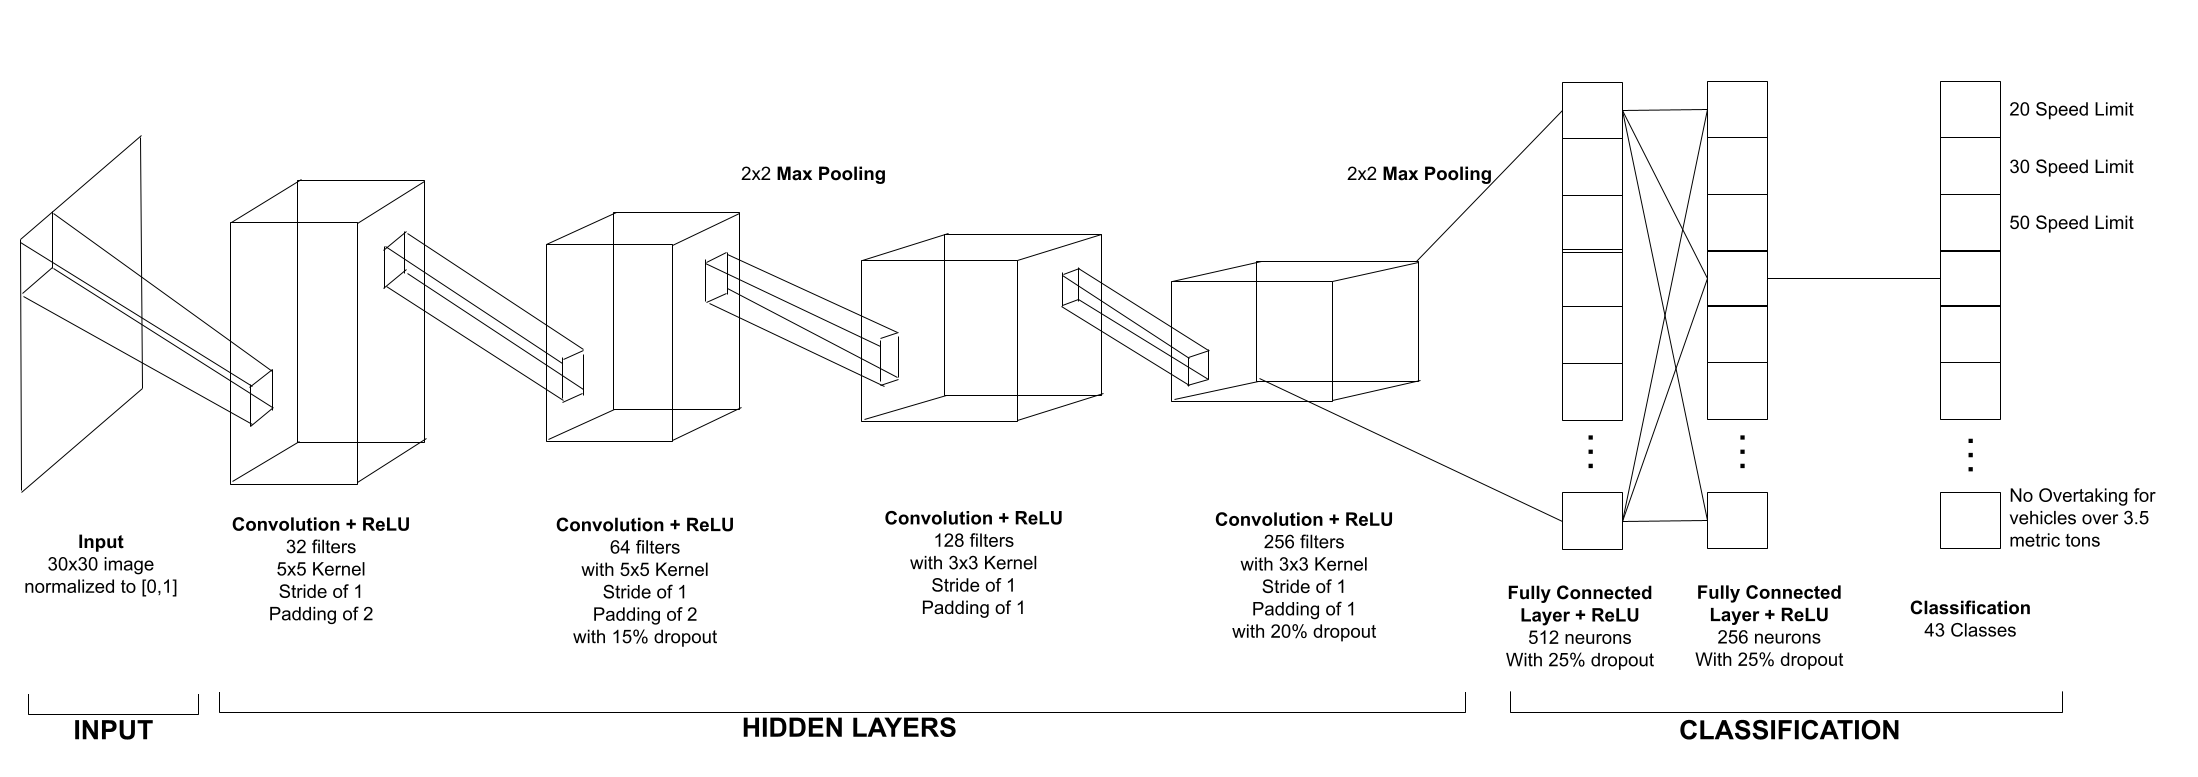
\includegraphics[width=0.5\linewidth]{CNN Schematic.png}
    \caption{Schematic of CNN Model}
    \label{fig:enter-label}
\end{figure}
\label{others}
\subsection{Input Layer} 
The model accepts RGB images resized to 30x30, normalized to have values in the range [0,1]. This preprocessing ensures consistency across the dataset and improves convergence during training.

\subsection{Convolutional and Fully Connected Layers}
This project employs a Convolutional Neural Network (CNN) due to its ability to scale large datasets. This model is consistent of 4 convolutional layers. The first layer is 5x5 with 32 filters, followed by ReLU activation. The second layer is 5x5 with 64 filters, ReLU activation, 2x2 max pooling and a dropout rate of 0.15. The third layer is 3x3 with 128 filters, followed by ReLU. The last layer is a 3x3 with 256 filters, ReLU activation, 2x2 max pooling and a dropout rate of 0.2. Subsequently, there are 2 fully connected layers. The first layer has 512 neurons, ReLU activation, and a dropout rate of 0.25. Lastly, there is a layer with 256 neurons, ReLU activation and a dropout rate of 0.25. 

%\begin{itemize}
   % \item Conv1: A 5x5 convolutional layer with 32 filters, followed by ReLU activation. The first convolution layer extracts low-level features like edges and corners from the input image.  
  %  \item Conv2: A 5x5 convolutional layer with 64 filters, followed by ReLU activation and 2x2 max pooling. Additionally, there is an applied dropout rate of 0.15. Dropout was applied in order to mitigate overfitting by randomly deactivating nodes during training. This layer builds on the previous features, capturing mid-level spatial patterns and reducing spatial dimensions.
   % \item Conv3: A 3x3 convolutional layer with 128 filters, followed by ReLU activation. This layer further refines the learned features with higher granularity, capturing more complex patterns.
  %  \item Conv4: A 3x3 convolutional layer with 256 filters, followed by ReLU activation and 2x2 max pooling. A dropout rate of 0.20 is applied. This layer focuses on high-level abstractions of the input, further reducing spatial dimensions.
%\end{itemize}

%\subsection{Fully Connected (FC) Layers}
%\begin{itemize}
   % \item FC1: A dense layer with 512 neurons, followed by ReLU activation and a dropout rate of 0.25. This layer connects the spatially reduced feature maps to a high-dimensional representation of the data.
   % \item FC2: A dense layer with 256 neurons, followed by ReLU activation and a dropout rate of 0.25. This layer further condenses the learned features.
%\end{itemize}

\subsection{Output Layer}
The output layer consists of a dense layer with 43 neurons, corresponding to the number of traffic sign classes in the GTSRB system. A softmax activation function is applied, ensuring the output represents probabilities for each class.

\subsection{Training Setup and Hyperparameters}
Various iterations were conducted to find the optimal hyperparameters for this model. The Adam Optimizer is used with a learning rate of 0.001. A cross entropy loss is employed, and the training uses a batch size of 128 and 30 epochs. 
%\begin{itemize}
 %   \item The Adam optimizer is used with a learning rate of 0.001.
  %  \item Cross-entropy loss is employed, given its suitability for multi-class classification tasks.
   % \item Batch Size = 128 
    %\item Number of Epochs = 30
%\end{itemize}
% The model achieved strong training and validation performance. After training for 30 epochs: 
%\begin{itemize}
  %  \item Training Accuracy: 95.95\%
%    \item Validation Accuracy: 96.21\%
%\end{itemize}

%The gap between training and validation accuracy indicates good generalization, suggesting that the model effectively avoided overfitting due to the use of dropout. Analyzing the performance on the validation set, most errors occurred in low-light conditions or blurred images and signs with similar visual structures (ex. Speed limits with different values).  

%The architecture achieves a strong balance between complexity and performance. Its relatively shallow depth ensures computational efficiency while its sufficient capacity captures the nuances of traffic sign patterns, enabling it to generalize well across diverse conditions. It has proven to be effective in classifying traffic signs with a high accuracy making it suitable for real-life systems in vehicles.

\section{Baseline Model}
For the baseline, a Support Vector Machine (SVM) was trained by employing preprocessed grayscale images resized to 32x32 pixels. The SVM with a linear kernel and a regularization parameter C = 1.0 thus achieving a 84.56\% accuracy. This simple and efficient model serves as a solid benchmark for assessing more advanced models such as CNNs, with room for improvement with respect to hyperparamters and non linear kernels. 
%For our baseline model, we trained a Support Vector Machine (SVM) classifier using the preprocessed dataset. SVM is a supervised learning algorithm that categorizes data by identifying a hyperplane that best separates different classes in a high-dimensional space. In binary classification, this hyperplane acts as the dividing line, while in multiclass scenarios, the SVM creates multiple hyperplanes to separate the classes pairwise. The support vectors, those data points closest to the hyperplane, are crucial for defining this boundary and influencing the model’s predictions.

%We chose the SVM as our baseline model because of its simplicity and efficiency and it is a solid foundation for assessing the enhancements offered by more complex models like CNNs. %Having a reliable benchmark allows us to appreciate the improvements brought by advanced techniques, while also shedding light on the strengths and limitations of simpler methods.

%For our implementation, we opted for a linear kernel for computational simplicity. We set the regularization parameter C to 1.0, which was a good balance between achieving a smooth decision boundary and minimizing classification errors on the training data. Additionally, we used a default tolerance of 0.0001 for optimization convergence.

%To prepare the data, we resized all images to 32x32 pixels and converted them to grayscale to simplify the data. Each grayscale image was flattened into a one-dimensional vector, allowing the SVM to process the images as structured feature sets. We also standardized these vectors to normalize pixel intensity ranges, which helped the model converge more smoothly.

%We evaluated the SVM’s performance using accuracy, a clear and straightforward metric that aligns with our goal of effectively classifying traffic signs. To gain deeper insights, we created a confusion matrix that showed how the model performed across individual classes and highlighted any patterns in misclassifications, providing valuable direction for future improvements.

%The SVM achieved an accuracy of 84.56\%, demonstrating that even a basic linear model can uncover meaningful patterns in the traffic sign data. While this serves as a solid benchmark, there’s definitely room for improvement by exploring non-linear kernels or tweaking hyperparameters like C. A detailed diagram of the SVM workflow is shown in Figure 4.
\begin{figure}[h]
    \centering
    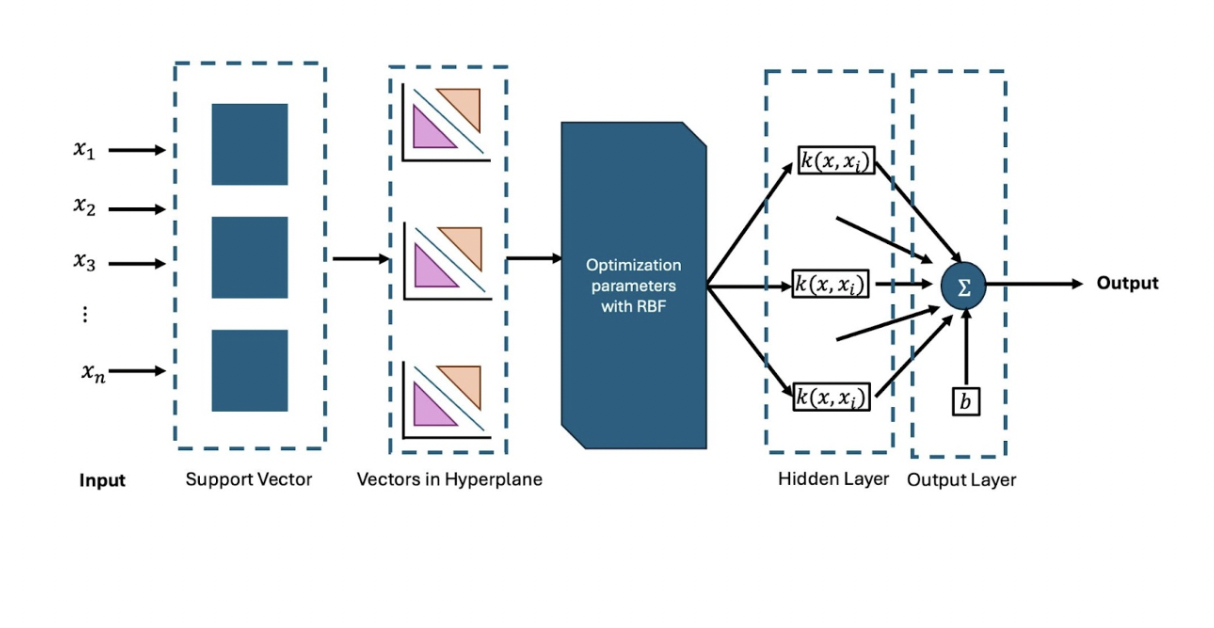
\includegraphics[width=0.5\linewidth]{SVM Baseline Model.png}
    \caption{Schematic of Baseline Model}
    \label{fig:enter-label}
\end{figure}

We also took a closer look at the model’s predictions to understand its strengths and weaknesses. The SVM performed well with traffic signs that had distinct features, such as stop and speed limit signs. However, it struggled with signs that were visually similar, like yield and caution signs, where subtle differences in shape or color led to misclassifications. These challenges highlight the limitations of using SVMs for datasets with nuanced inter-class differences and underscore the need for more advanced methods like CNNs.

\section{Quantitative Results}
This section describes the quantitative measures used to evaluate the performance of our final model using several metrics. 
\subsection{Accuracy}
Our model achieved an accuracy of 95.92\% on the test set, indicating its strong capability in recognizing most traffic signs correctly. While accuracy gives a general sense of performance, it doesn’t account for class imbalances. This is crucial since certain traffic signs, like stop or yield signs, carry more significance in real-world situations. High accuracy suggests that the model can be generally trusted, but a deeper look into other metrics is necessary to assess its class-specific performance.
\subsection{Precision and Recall}
Precision and recall are crucial metrics, especially when misclassification consequences vary. Precision indicates the proportion of true positives among predicted positives, while recall measures the proportion of actual positives correctly identified. For instance, low precision for a stop sign may cause unnecessary braking, whereas low recall for a yield sign could lead to collisions. Our analysis shows an average precision of 95\% and recall of 94\%, demonstrating the model’s effectiveness in minimizing misclassifications and identifying critical traffic signs. In autonomous driving, high precision ensures reliability, and high recall reduces the risk of missing key signs.

\subsection{F1 Score}
The F1 score, which is the harmonic mean of precision and recall, serves as a balanced metric, especially useful when dealing with imbalanced datasets. Our model achieved an average F1 score of 0.935, reflecting strong and consistent performance across various classes. In real-world applications such as self-driving cars, achieving a balance between precision and recall is essential. Overemphasizing recall could lead to false alarms for signs that aren’t present, while focusing solely on precision might result in missing critical signs. The F1 score allows us to assess the model's robustness in navigating these trade-offs.

\subsection{Confusion Matrix}
The confusion matrix helps to visualize the model's prediction outcomes. It provides a breakdown of correct and incorrect predictions for each class, highlighting which traffic signs are frequently misclassified. For instance, our analysis revealed that the model sometimes confused caution signs with yield signs due to their similar shapes and colors. This insight is crucial for identifying the model's limitations and guiding future improvements. If the model is intended for use in self-driving cars, enhancing its ability to differentiate visually similar signs will be vital, as such errors could have serious implications in traffic scenarios. Additionally, understanding these misclassification patterns can inform future training strategies, such as gathering more diverse samples of misclassified signs or employing data augmentation techniques to improve generalization across similar classes.


\section{Qualitative Results}
To illustrate the performance of our Traffic Sign Recognition (TSR) model with qualitative results, we present several sample predictions that highlight its strengths and areas for improvement. The samples include correctly and incorrectly classified traffic signs, emphasizing patterns in the model's performance.
\subsection{Correct Classification} 

\begin{figure}[h]
    \centering
    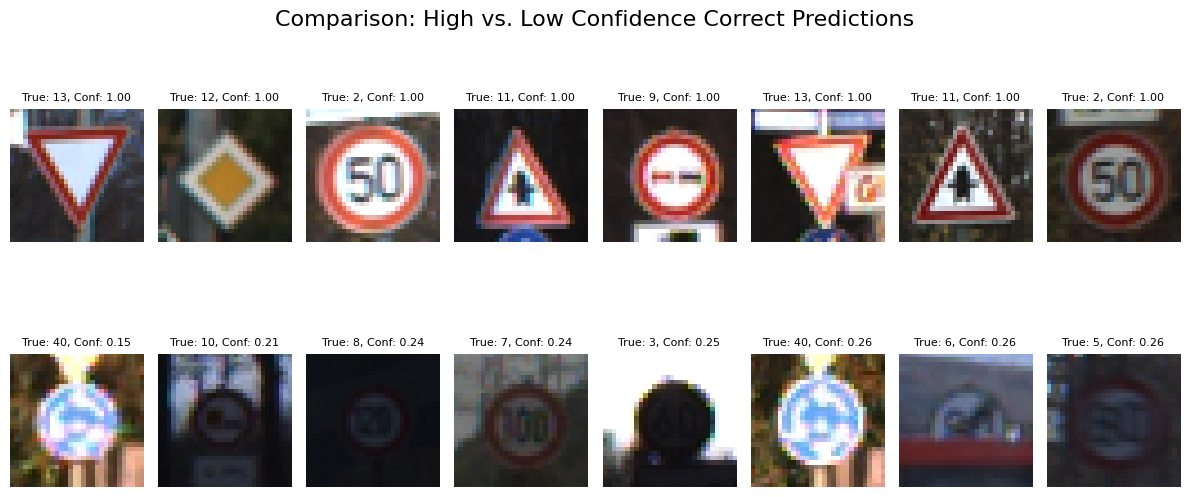
\includegraphics[width=0.5\linewidth]{Comparison of confidence.png}
    \caption{Correctly Classified Samples, High (top) vs. Low (bottom) Confidence}
    \label{fig:enter-label}
\end{figure}

    The model correctly identifies signs with clear and unobstructed signs. For example, “Yield” signs (class 13) under bright daylight conditions were classified with confidence scores of 100\%. The high contrast between the red border and white centre enabled the model to easily extract distinguishing features. Additionally, a "Speed limit (50km/h)" sign (class 2) with no occlusions was correctly predicted with a confidence of 100\%. The clear visibility of text and numbers contributed to the accurate classification.
    As seen in Figure 5, signs with slight occlusions are identified correctly but with extremely low confidence. The model’s ability to generalize to partial patterns indicates that the convolutional layers effectively learned spatial hierarchies.

\subsection{Misclassifications}
    A majority of the images that were misclassified were blurred or low-light. As seen on the left 16 images in Figure 6, 14 out of the 16 images are low-light and difficult to view. For example, the model misclassified an extremely dark image of a “Traffic lights” sign (class 26) as a “General caution” sign (class 18) with 100\% confidence. The model struggled to discern key features due to insufficient contrast and clarity.
    
    Classes that share similar shapes and text layouts, make it challenging for the model to differentiate when distortions are present and these photos seem to be misclassified with intense confidence. This happens most often and expectedly for circular speed limit signs as the text layout may make it difficult for the model to read. For example, a "Speed limit (80km/h)" sign (class 5) was misclassified as "Speed limit (60km/h)" (class 3) with a confidence score of 68\%. As well as speed limits, this is an occurrence for any signs of similar shapes. For example, the “Road narrows on right” sign (class 24) was mistaken for the “General caution” (class 18) sign with 96\% confidence as they both share an upward triangular shape. 
    %\begin{figure}[h]
       % \centering
        % 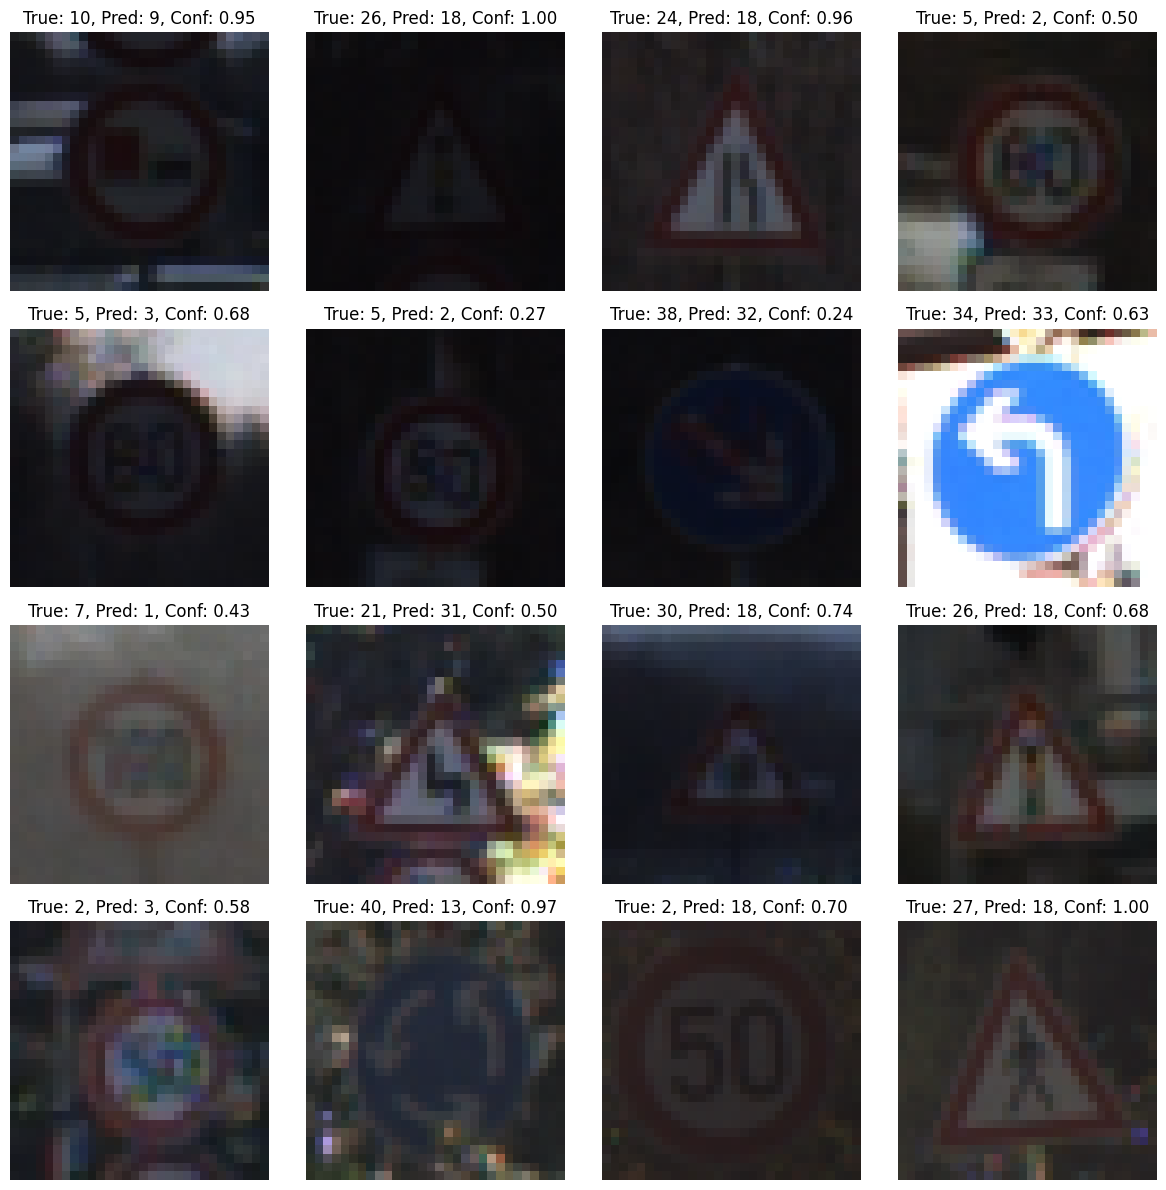
\includegraphics[width=0.3\linewidth]{Misclassified1.png}
       %  \caption{Examples of Misclassified Signs with True Class, Predicted Class, and Model Confidence}
        % \label{fig:enter-label}
    %\end{figure}
   % \begin{figure}[h]
       % \centering
       % 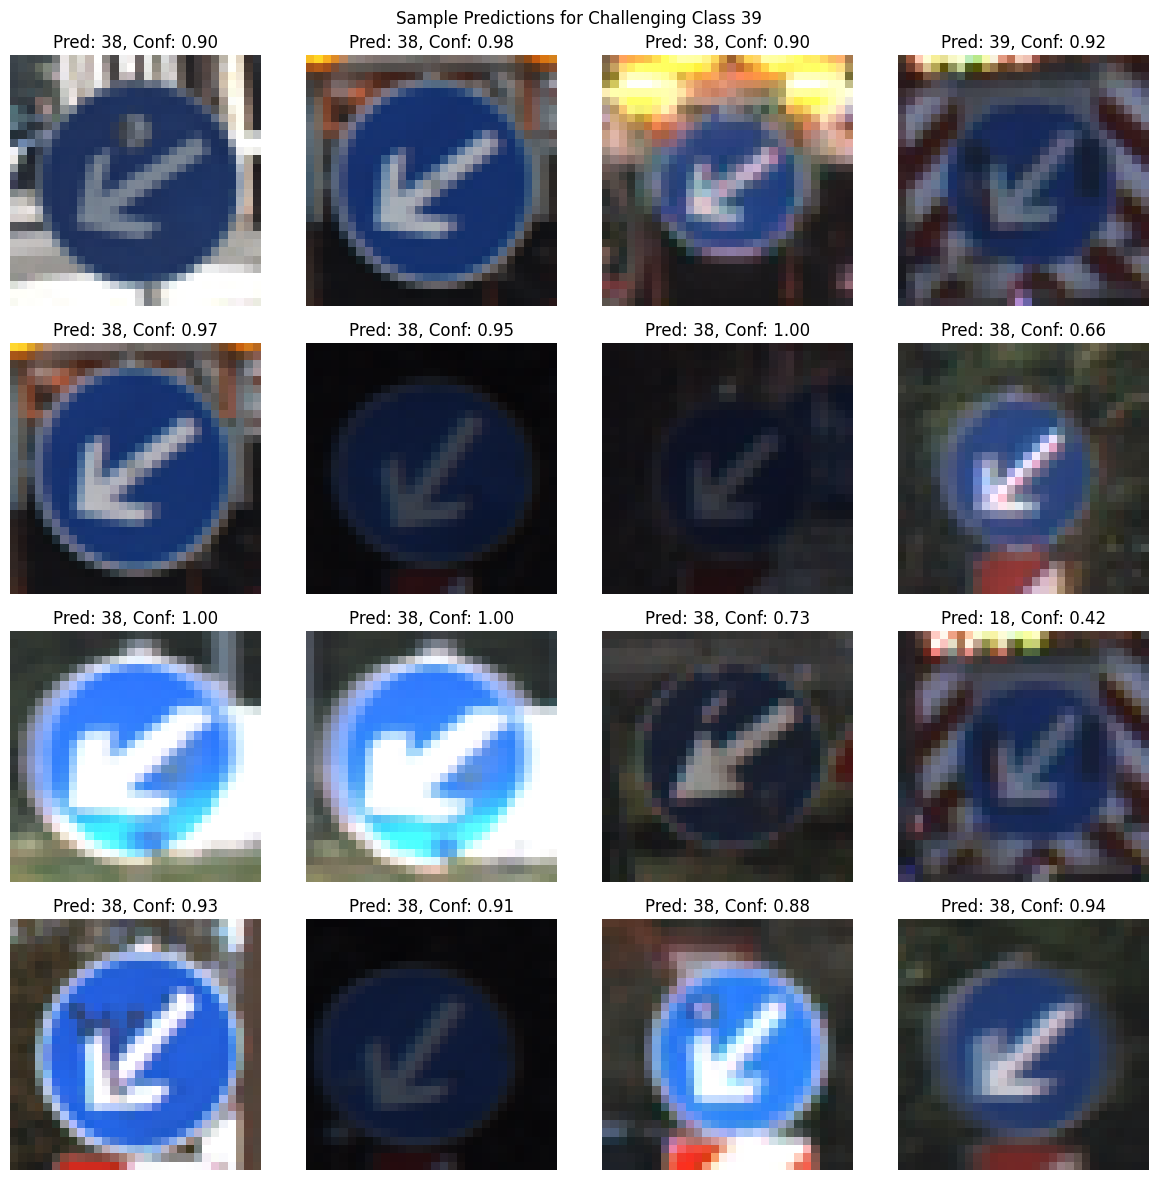
\includegraphics[width=0.3\linewidth]{Misclassified2.png}
      %  \caption{Examples of Most Misclassified, Class 39 (“Keep left”), with Model Confidence}
     %   \label{fig:enter-label}
   % \end{figure}
   \begin{figure}[h]
       \centering
       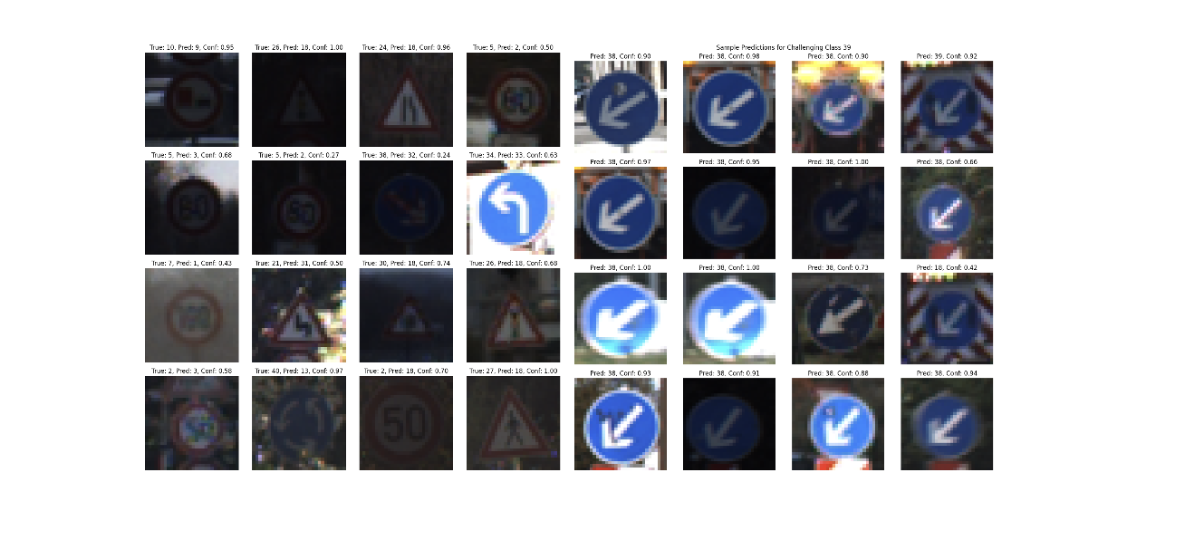
\includegraphics[width=0.5\linewidth]{Missclassified Images .png}
       \caption{Missclassified Images}
       \label{fig:enter-label}
   \end{figure}

    The model also commonly confused directional signs. For example, the “Keep left” sign (class 39) was highly misclassified with an accuracy of 58.62\%. As seen on the right 16 images of Figure 6, it is usually confused as the “Keep right” sign (class 38) with high confidence. This is most likely due to data augmentations/transforms that affected the training and validation dataset. Since the model was trained with data that had random horizontal flipping, it is likely that it learnt on misrepresented directional signs and as a result will misclassify left and right signs.

\subsection{Model Takeaways}

The qualitative results align with the quantitative metrics, showing that the model performs exceptionally well on clean, well-lit images with minimal distortion or occlusion. However, it faces challenges with low-light or blurred conditions, as they reduce feature clarity which impacts model performance, and visually similar classes, where high class similarity and distortions can lead the model to confusion. The model’s qualitative performance suggests potential improvements through techniques like:
\begin{itemize}
    \item Data Augmentation Changes: Introducing motion blur, low-light conditions, and occlusions during training to enhance robustness. Removing flipping and rotation augmentations for directional signs.
    \item Effective Convolution Layer Mechanisms: Incorporating convolution layers to pay attention/focus on critical regions of the image for better class differentiation.
\end{itemize}
Overall, these results demonstrate the model's ability to generalize well in most scenarios, while also providing insight into areas where additional optimization could enhance performance.


\section{Evaluate Model on New Data}

To ensure that the results accurately represent the model's performance on new, unseen data, we implemented several strategies throughout the development and evaluation process:

\subsection{Data Splitting}

We divided the dataset into training, validation, and test sets into 70\%, 15\%, and 15\% respectively. The training set was used to optimize the model's parameters, the validation set for hyperparameter tuning, and the test set for final evaluation. This split ensures that the model's performance on unseen data can be reliably assessed. Additionally, the test set was not exposed during training or validation, preventing any data leakage that could inflate the model's performance.

\subsection{Data Augmentation}

We employed extensive data augmentation techniques to simulate real-world variability in traffic signs. These included:
\begin{itemize}
    \item Random rotations and translations to mimic variations in camera angles
    \item Brightness adjustments to account for changes in lighting conditions
    \item Adding random noise to simulate sensor inaccuracies
    \item Random cropping and flips to introduce perspective distortions
\end{itemize}

These augmentations increased the diversity of the training data, making the model more robust to variations encountered in real-world scenarios. This helped reduce overfitting and improved generalization to new data.

\subsection{Dropout}

Dropout was integrated into the architecture at multiple points, with rates of 0.15, 0.20, and 0.25 for convolutional and fully connected layers. Dropout helps prevent the model from relying too heavily on specific neurons by randomly deactivating them during training. This forces the model to learn more generalized features, thereby enhancing its performance on unseen data.

\subsection{Baseline Model}

To evaluate the effectiveness of our final model, we first implemented a baseline model with a simple architecture. The baseline model achieved limited accuracy due to its inability to capture the nuances of traffic sign patterns. This comparison highlighted the improvements brought by our deeper and more robust CNN architecture, augmented training data, and advanced optimization techniques.

\subsection{Evaluation Metrics}

We used multiple evaluation metrics to assess the model's performance:
\begin{itemize}
    \item Validation Accuracy: The final validation accuracy of 96.21\% demonstrated the model's ability to generalize well during training
    \item Test Accuracy: A test accuracy of 95.92\% indicated that the model maintained its performance on entirely unseen data.
    \item Confusion Matrix: We analyzed a confusion matrix to identify specific classes where the model struggled. Most errors occurred in low-light images, blurred signs, or signs with similar visual structures, such as speed limits with different values.
    \item F1 Score: The F1 score was calculated to measure the balance between precision and recall across all traffic sign classes, ensuring no particular class dominated the
    
\end{itemize}

\subsection{Real-World Testing}

Beyond the dataset, the model was tested on a small set of new traffic sign images collected from real-life photos. These images included scenarios like partial occlusions and adverse weather conditions, but most importantly these were photos taken of Toronto traffic signs. This was done in order to test the system's effectiveness at classifying global traffic signs that differ from the original dataset, determining whether the system is universal. The model's consistent performance reinforced its robustness to real-world challenges.
\newpage
\begin{figure}[h]
    \centering
    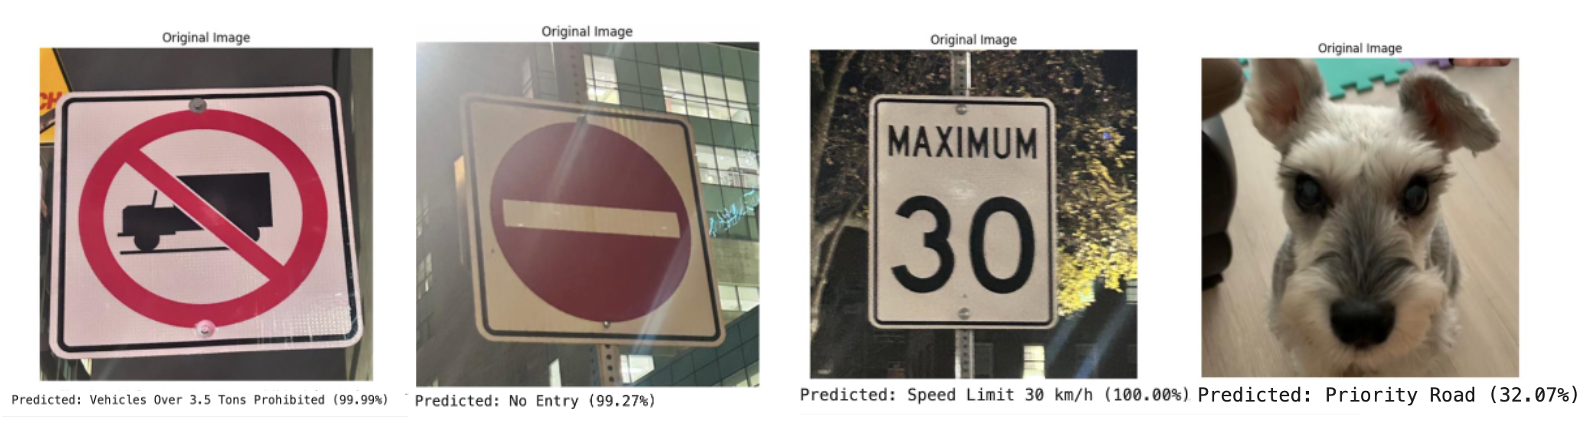
\includegraphics[width=0.5\linewidth]{classificationstext.png}
    \caption{Results of Data with Unseen Data}
    \label{fig:enter-label}
\end{figure}

\section{Discussion}

\begin{figure}[h]
    \centering
    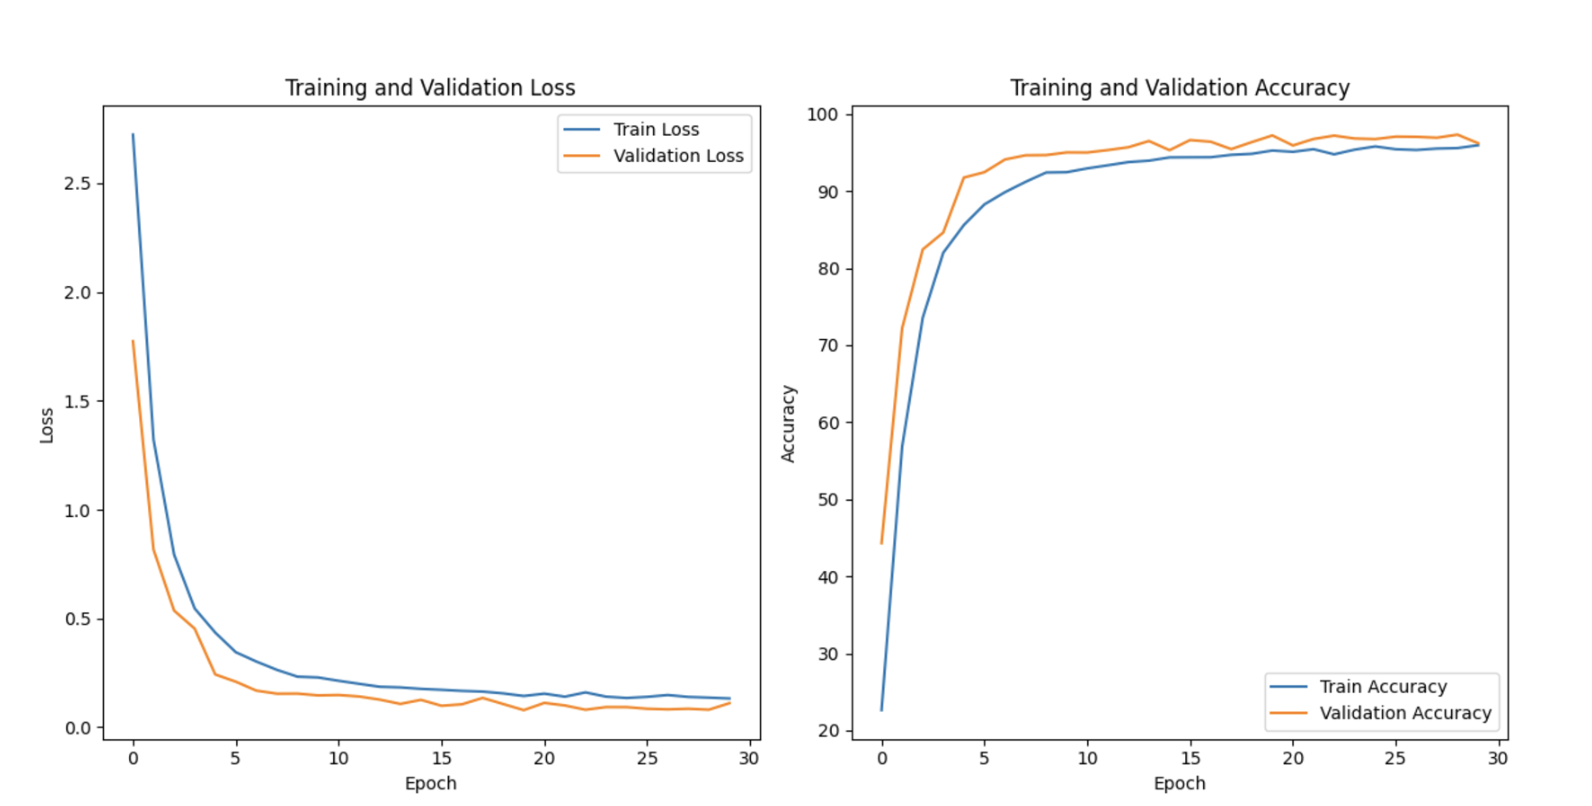
\includegraphics[width=0.5\linewidth]{Validation and Training.png}
    \caption{Training and Validation Loss (left) and Accuracy (right) over 30 Epochs}
    \label{fig:enter-label}
\end{figure}

The Traffic Sign Recognition system demonstrated strong performance with a training accuracy of 95.95\% and a validation accuracy of 96.21\%. Initially, the model performed too well on the dataset having reached close to 100\% training accuracy, highlighting that the data being fed into it was too easy. This would most likely lead to the model ineffectively classifying signs with present obstructions. To address this, the team applied extensive data augmentation techniques, including rotations, brightness adjustments, zooms, noise, cropping, translations, and flips. These augmentations increased the difficulty of the input data, challenging the model to generalize more effectively. This effort brought the test accuracy to 95.92\% and improved its robustness under diverse conditions.

We observed that CNNs are apt at recognizing distinct shapes and patterns, such as the circular speed limit signs, octagonal stop signs, triangular yield signs, and text or image layout. The original dataset's clean and distinct visuals allowed the model to quickly and accurately classify signs. By introducing distortions through augmentation, the learning process became more challenging, forcing the model to adapt and learn features more resiliently.

While the dropout layers reduced overfitting, the primary challenges arose in scenarios with low-light conditions, motion blur, or visually similar signs, such as speed limits with varying numerical values. Future work could focus on adding more advanced augmentations or improving the dataset balance to mitigate these limitations. Additionally, using higher-resolution inputs or pre-trained feature extractors might further enhance the model's ability to handle complex and nuanced visual patterns.

The gap between training and validation accuracy indicates good generalization, suggesting that the model effectively avoided overfitting due to the use of dropout. Analyzing the performance on the validation set, most errors occurred in low-light conditions or blurred images and signs with similar visual structures (ex. Speed limits with different values).  

The architecture achieves a strong balance between complexity and performance. Its relatively shallow depth ensures computational efficiency while its sufficient capacity captures the nuances of traffic sign patterns, enabling it to generalize well across diverse conditions. It has proven to be effective in classifying traffic signs with a high accuracy making it suitable for real-life systems in vehicles. 


\section{Ethical Considerations}
\subsection{Potential Ethical Issues:} 
\begin{itemize}
    \item Safety and accuracy: The model must be able to identify traffic signs with extremely high accuracy regardless of different real-world and environmental factors to ensure the safety of its users.
    \item Privacy: Care must be taken to ensure that no faces or license plates are accidentally caught in any of the input images fed to the model to ensure that there is no breach of privacy.
    \item Bias in training data: The GTSRB dataset predominantly contains German traffic signs, which may not represent traffic signs from other countries or regions. Thus, deploying the model in diverse geographical locations could lead to biases, misinterpretations, or failures.
\end{itemize}
\subsection{Model Limitations:}  
\begin{itemize}
    \item Accuracy in Adverse Conditions: The model's performance may degrade under poor lighting, occlusion, or extreme weather conditions not well-represented in the dataset. This limitation could lead to errors in real-world scenarios.
    \item Class Imbalance: Some traffic sign classes are underrepresented in the GTSRB dataset. This imbalance may cause the model to perform poorly on these less-common classes, leading to a potential safety risk.
    \item Generalization: The model was trained specifically on German traffic signs, meaning it may not generalize well to traffic signs from other countries with different designs, symbols, or languages.
    \item Dynamic environments: Real-world traffic scenarios often involve dynamic elements such as moving vehicles, pedestrians, and environmental distractions. The model, which was trained on static images, may not handle these complexities effectively.
\end{itemize}

\subsection{Training Data Limitation:}
\begin{itemize}
    \item Dataset diversity: The GTSRB dataset may not fully capture the variety of real-world conditions, such as weather variations, damaged or obscured signs, or signs affected by vandalism.
    \item Data augmentation limitations: While augmentation helps improve diversity, it cannot fully replicate real-world scenarios, potentially leaving gaps in the model's robustness.
\end{itemize}
\section{Project Difficulty}
This model presents challenges that make it relatively difficult to recognize signs via data augmentation with the objective of generalizing the model. Firstly, the problem itself is inherently complex as TSR systems should be able to classify traffic signs through adverse conditions. This includes lighting changes, obstructed views and weather impacts. Furthermore, traffic signs follow similar patterns and colours, thus making classification relatively difficult. Due to the real world applications with fast-moving objects as most cars are in morition, this already adds a level of complexity that static datasets cannot exhaustively simulate.

The chosen dataset also presents a variety of challenges such as imbalanced class distributions in the GTSRB dataset, and therefore the model may face difficulties in learning more rare classes as they may not be encountered as frequently. The GTSRB dataset is also comprehensive in German traffic signs; it may not be able to be universally applied.

Due to the safety implications of a TSR model, the accuracy must be incredibly high and must also work efficiently to make real time predictions and classifications while the car is in motion.

With respect to the model itself, several augmentation layers have been added including cropping, jitter, noise, zoom, horizontal flip and rotation of the inputted image to make the model robust at classifying signs. Despite all the augmentations added to the model, it retains a high accuracy rate.



\newpage


\label{last_page}

\bibliography{APS360_ref}
\bibliographystyle{iclr2022_conference}

\end{document}
